% !TEX root = sd_tokenskip_paper.tex
% Main paper draft.
\documentclass[runningheads]{llncs}

\usepackage[T1]{fontenc}
\usepackage{amsmath}
\usepackage{graphicx}
\usepackage{booktabs}
\usepackage{array}
\usepackage{float}
\usepackage{xcolor}
\definecolor{emailblue}{RGB}{88,128,164}
\usepackage[colorlinks=true,linkcolor=black,citecolor=black,urlcolor=emailblue]{hyperref}
\setlength{\emergencystretch}{2em}

\newcommand{\emailaddress}[1]{\href{https://mail.google.com/mail/?view=cm\&fs=1\&to=#1}{\texttt{#1}}}

\begin{document}
\raggedbottom

\title{\texorpdfstring{\parbox{\textwidth}{\raggedright
Evaluating SD-TokenSkip Against Fixed Compression Ratios}}
{Evaluating SD-TokenSkip Against Fixed Compression Ratios}}

\titlerunning{Evaluating SD-TokenSkip}

\author{Vu Dinh Hong\inst{1} \and
Chau Pham Tuan Kiet\inst{2} \and
Nguyen Ba Hung\inst{2}}

\authorrunning{Vu Dinh Hong, Chau Pham Tuan Kiet, and Nguyen Ba Hung}

\institute{\textsuperscript{1} Natural Language Processing and Knowledge Discovery Research Group, Faculty of Information Technology, Ton Duc Thang University, Ho Chi Minh City, Vietnam\\
\textsuperscript{2} Faculty of Information Technology, Ton Duc Thang University, Ho Chi Minh City, Vietnam\\
\emailaddress{vudinhhong@tdtu.edu.vn}, \emailaddress{523k0011@student.tdtu.edu.vn}, \emailaddress{523k0006@student.tdtu.edu.vn}\\
Corresponding author: \emailaddress{523k0011@student.tdtu.edu.vn} (Chau Pham Tuan Kiet),\\
\emailaddress{523k0006@student.tdtu.edu.vn} (Nguyen Ba Hung)}

\maketitle

\begin{abstract}
TokenSkip exposes a control for shortening chain-of-thought traces. We ask whether a question-dependent rule improves the accuracy--length trade-off over a fixed ratio. We evaluate a frozen six-feature router, SD-TokenSkip, and six fixed ratios on the same 1,319 GSM8K questions with Qwen2.5-3B-Instruct and 7B-Instruct. The router reaches 82.34\% accuracy at 264.40 mean reasoning tokens on 3B and 89.39\% at 230.90 tokens on 7B. Fixed ratios 0.9 on 3B and 0.7 on 7B give slightly higher observed accuracy and shorter traces. Paired accuracy intervals contain zero for both comparisons, while fixed 0.7 saves 6.28\% tokens on 7B (95\% interval 4.75--7.76\%). The score's AUROC for compression-induced errors varies from 0.588 to 0.669 on 7B, depending on the ratio. Neither adapter provides evidence of a reliable adaptive advantage.
\keywords{Chain-of-thought \and TokenSkip \and adaptive inference \and GSM8K}
\end{abstract}

\section{Introduction}
Chain-of-thought (CoT) prompting can improve arithmetic reasoning \cite{wei2022,kojima2022}, but generating intermediate steps consumes decoding tokens. TokenSkip trains models to produce shorter reasoning traces under a requested compression ratio \cite{tokenskip}. A fixed ratio is simple to deploy. An input-dependent rule is useful if it can identify where changing the ratio improves the trade-off between accuracy and generated length.

We compare a frozen router that uses six question features with all six fixed settings under a common inference protocol. We ask whether its score predicts loss under compression and whether its assignments improve on shuffled assignments with the same ratio frequencies. We evaluate the frozen router on the full GSM8K test set.

The study contributes a question-aligned evaluation with fixed-ratio and allocation controls, a diagnostic distinction between difficulty and sensitivity to compression, and an analysis of policy and baseline-selection instability. These findings concern the tested six-feature router and adapters; they do not imply that all adaptive compression methods are ineffective. Our working hypothesis is that input structure can indicate where a shorter reasoning trace is less likely to lose correctness. We test this as an empirical question, rather than assuming that longer or structurally complex questions always require a larger ratio.

\section{Related work}
TokenSkip learns to omit less useful reasoning tokens at a requested ratio \cite{tokenskip}. TALE estimates token budgets for prompts \cite{tale}, while CoT-Valve controls reasoning length through parameter-space tuning \cite{cotvalve}. C3oT learns from long and short rationales, and C3oT-Adapt selects an appropriate compression level using accuracy during preparation of its training data \cite{c3ot}. L1 trains a model to follow requested length constraints \cite{l1}. O1-Pruner uses length-aware fine-tuning for shorter reasoning traces \cite{pruner}.

Several methods allocate more computation where it is likely to help. Snell et al. study prompt-dependent search and revisions under matched inference budgets \cite{snell}. Damani et al. estimate marginal returns to computation and use those estimates to allocate decoding effort \cite{damani}. DAST learns to adjust reasoning length with difficulty-aware training \cite{dast}. AdaCoT learns when to trigger CoT with reinforcement learning \cite{adacot}. We use existing TokenSkip adapters and study the choice among their discrete ratios.

\section{Question-based ratio selection}
\subsection{Frozen SD-TokenSkip policy}
Selective Difficulty-Conditioned TokenSkip (SD-TokenSkip) runs before generation (Fig.~\ref{fig:architecture}). It counts question tokens, numeric spans, arithmetic operators, clause connectors, number--unit pairs, and comparison markers. It standardizes these counts using the fit partition and averages the six standardized values. Fit-set quantiles define ten score bins. Bins 1--5, 6--7, and 8--10 form the \emph{easy}, \emph{medium}, and \emph{hard} groups. These names refer to score bands, not validated difficulty labels.

\begin{figure}[!htbp]
\centering
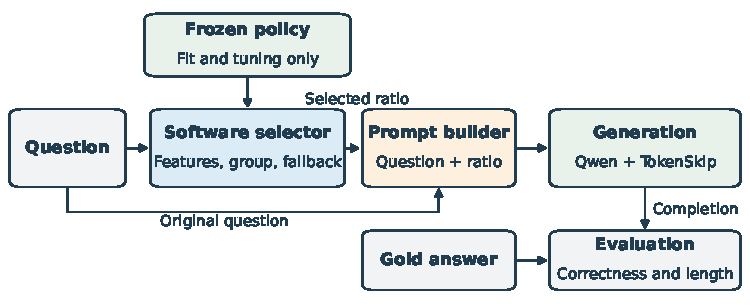
\includegraphics[width=\linewidth]{figures/matched_architecture.pdf}
\caption{The selector runs outside the model and passes a ratio to the prompt builder. The evaluation stage receives the gold answer after generation.}
\label{fig:architecture}
\end{figure}

For a partition, let $A$ be accuracy in percentage points and $\bar L_1$ the mean CoT length at $\gamma=1.0$. The development procedure scores policies by
\begin{equation}
U=A+\lambda R,\qquad R=100\left(1-\frac{\bar L}{\bar L_1}\right).
\label{eq:utility}
\end{equation}
The original policy uses $\lambda=0.1$, which values a ten-point increase in percentage token reduction as one point of accuracy. We treat this as a design preference and vary it in the development analysis.

Each group chooses a ratio from $\Gamma=\{0.5,0.6,0.7,0.8,0.9,1.0\}$ using its contribution to Eq.~\ref{eq:utility}. On the fit partition, the contribution is $100C_g/N-100\lambda T_g/B$, where $C_g$ and $T_g$ are correct answers and total tokens for eligible questions in group $g$, $N$ is the full fit size, and $B$ is the total baseline length at $\gamma=1.0$ across that partition. Inputs outside the 1st--99th percentile fit bounds of any feature receive $\gamma=1.0$. Groups with fewer than 30 eligible fit examples also default to 1.0.

The original calibration used 540 fit, 180 tuning, and 180 validation questions from the GSM8K training split \cite{gsm8k}. Fit outcomes determined candidate maps. Tuning selected among four candidates that use either three or six structural features and differ in grouping, allowed mappings, and fallback. The six-feature policy had the highest tuning utility for both models. Its frozen easy/medium/hard ratios are $0.7/0.8/1.0$ for 3B and $0.9/0.5/0.8$ for 7B. We retain these assignments in the test comparison.

\section{Evaluation}
\subsection{Matched inference on GSM8K}
We use Qwen2.5-3B-Instruct and Qwen2.5-7B-Instruct \cite{qwen25} and their corresponding GSM8K TokenSkip adapters \cite{tokenskip}. On one RTX 3090, we generate responses for all 1,319 questions at each of six fixed ratios and with frozen SD, yielding 18,466 recorded generations. All conditions share the model and adapter revisions, prompt template, FP16 precision, SDPA, greedy decoding, batch size 16, seed 42, and a limit of 512 new tokens. The prompt appends the TokenSkip ratio marker below 1.0. At 1.0 it omits the marker while retaining the merged adapter. The official \href{https://github.com/hemingkx/TokenSkip/blob/main/get_llamafactory_input.py}{data preparation script} uses the original input unchanged for its 1.0 branch and appends markers for compressed branches. We did not verify the exact training files used to produce each released adapter. Native EOS termination matched the previous stopping helper in a same-batch pilot of three questions per model.

Accuracy uses the archived numeric answer extraction and scoring functions. We tokenize the completion prefix before the literal separator \texttt{The final answer is:} preceded by two line breaks. If that separator is absent, the full completion is counted. We keep each output, score, and token count indexed by question. We use a paired question bootstrap with 20,000 resamples for differences and an exact two-sided McNemar test for accuracy. The two primary comparisons, one per model, use the fixed ratio selected by applying Eq.~\ref{eq:utility} to the original tuning partition. This selects $\gamma=0.5$ for both models. We apply Holm correction to those two tests and report the remaining comparisons as exploratory on a previously inspected public benchmark.

\subsection{Allocation and sensitivity analyses}
The full fixed grid lets us replay a ratio assignment by taking each question's recorded output at its assigned ratio. We compare SD replay with 10,000 shuffled assignments that retain its ratio histogram. A second shuffle keeps the 87 fallback positions fixed and permutes only the other assignments. We also compute the maximum utility attainable on the recorded grid by selecting the best observed outcome per question using the gold scores. That oracle measures headroom in the grid.

To separate difficulty from compression sensitivity, we measure the score's AUROC for errors at $\gamma=1.0$. For each lower ratio we also measure AUROC for switching from correct to wrong, restricting the denominator to questions answered correctly at 1.0.

\section{Results}
\subsection{Fixed ratios and frozen SD}
Tables~\ref{tab:matched} and~\ref{tab:matched7} give the complete grids separately. Relative to $\gamma=1.0$, SD uses 17.13\% fewer CoT tokens on 3B and 21.97\% fewer on 7B, with observed accuracy differences of $-0.83$ and $-2.43$ points. Compared with the tuning-selected $\gamma=0.5$, SD gains 7.51 accuracy points on 3B (95\% interval 5.31--9.70) and 3.79 on 7B (2.35--5.31), with Holm-adjusted $p<0.001$ for both. It also uses 55.93\% and 52.08\% more CoT tokens than fixed 0.5, respectively. The outcome at that aggressive setting is one part of the trade-off.

At the development weight $\lambda=0.1$, the paired utility difference SD minus fixed 0.5 is $+4.53$ (95\% interval $[2.36,6.75]$) for 3B and $+1.12$ ($[-0.35,2.63]$) for 7B. Utility summarizes a chosen accuracy--length preference and does not establish a universal trade-off advantage. This is especially important because the comparator is comparatively aggressive and because the benchmark has already been inspected.

Test-set utilities in Tables~\ref{tab:matched} and~\ref{tab:matched7} are descriptive. SD does not have the highest observed utility on either model: fixed 0.9 scores 84.86 versus 84.05 for SD on 3B, and 92.37 versus 91.58 on 7B. These test-inspected comparisons do not replace the tuning-selected primary comparison.

\begin{table}[H]
\caption{Qwen2.5-3B-Instruct: direct inference on 1,319 questions per condition; $U$ uses $\lambda=0.1$ and fixed 1.0 as the length reference.}
\label{tab:matched}
\centering\small
\begin{tabular}{l@{\hspace{8pt}}r@{\hspace{8pt}}r@{\hspace{8pt}}r@{\hspace{8pt}}r}
\toprule
Condition & Correct & Acc. (\%) & CoT tokens & $U$\\
\midrule
% Generated from matched inference analysis.
$\gamma=0.5$ & 987 & 74.83 & 169.56 \\
$\gamma=0.6$ & 1,012 & 76.72 & 199.92 \\
$\gamma=0.7$ & 1,058 & 80.21 & 233.03 \\
$\gamma=0.8$ & 1,080 & 81.88 & 251.22 \\
$\gamma=0.9$ & 1,096 & 83.09 & 262.52 \\
$\gamma=1.0$ & 1,097 & 83.17 & 319.04 \\
\midrule
SD-TokenSkip & 1,086 & 82.34 & 264.40 \\
\bottomrule

\end{tabular}
\end{table}

\begin{table}[H]
\caption{Qwen2.5-7B-Instruct: direct inference on 1,319 questions per condition; $U$ uses $\lambda=0.1$ and fixed 1.0 as the length reference.}
\label{tab:matched7}
\centering\small
\begin{tabular}{l@{\hspace{8pt}}r@{\hspace{8pt}}r@{\hspace{8pt}}r@{\hspace{8pt}}r}
\toprule
Condition & Correct & Acc. (\%) & CoT tokens & $U$\\
\midrule
% Generated from matched inference analysis.
$\gamma=0.5$ & 1,129 & 85.60 & 151.82 & 90.46 \\
$\gamma=0.6$ & 1,163 & 88.17 & 178.07 & 92.15 \\
$\gamma=0.7$ & 1,180 & 89.46 & 216.41 & 92.15 \\
$\gamma=0.8$ & 1,188 & 90.07 & 237.15 & 92.05 \\
$\gamma=0.9$ & 1,200 & 90.98 & 254.67 & 92.37 \\
$\gamma=1.0$ & 1,211 & 91.81 & 295.89 & 91.81 \\
\midrule
SD-TokenSkip & 1,179 & 89.39 & 230.90 & 91.58 \\
\bottomrule

\end{tabular}
\end{table}

Two fixed ratios examined after observing test results, 0.9 for 3B and 0.7 for 7B, give better observed accuracy and token means than SD in our own run (Fig.~\ref{fig:tradeoff}). Fixed 0.9 answers ten more 3B questions correctly and saves 0.71\% of SD's tokens (95\% interval $[-0.71,2.09]$). Its paired accuracy gain is 0.76 points (95\% interval $[-1.06,2.58]$, McNemar $p=0.456$). Fixed 0.7 answers one more 7B question correctly and saves 6.28\% of SD's tokens (95\% interval $[4.75,7.76]$). Its accuracy gain is 0.08 points ($[-1.29,1.44]$, $p=1.000$). These accuracy intervals allow differences in either direction. We did not specify an equivalence margin.

\begin{figure}[!htbp]
\centering
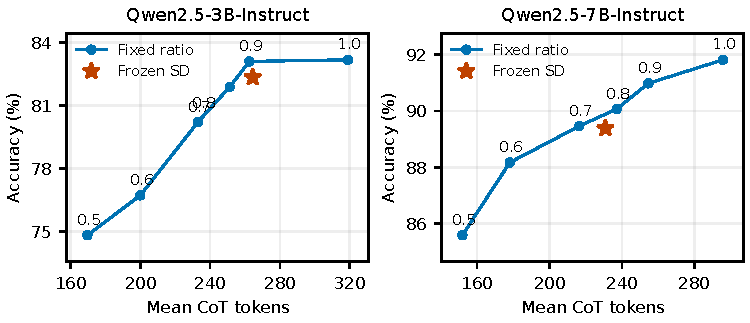
\includegraphics[width=\linewidth]{figures/matched_tradeoff.pdf}
\caption{Mean CoT length and accuracy for the two models. The points represent direct runs. The line connects the six tested fixed ratios to guide the eye.}
\label{fig:tradeoff}
\end{figure}

\subsection{Does the score identify useful ratio changes?}
With fallback held fixed, SD replay scores 0.87 utility points above the mean shuffle for 3B and 0.09 below it for 7B (unadjusted upper-tail permutation $p=0.044$ and $0.590$). Shuffling the entire histogram gives $p=0.069$ and $0.711$. The results give limited evidence for the 3B assignments and no consistent advantage across models. Batch composition changes between direct SD and grid replay: both have the same correct totals, but correctness changes on ten 3B questions and two 7B questions. The shuffle compares policies within replay.

The six-feature score has AUROC 0.660 and 0.656 for error at $\gamma=1.0$ on 3B and 7B. For compression loss among questions correct at 1.0, AUROC varies across the five lower ratios (0.631--0.654 on 3B and 0.588--0.669 on 7B). In particular, discrimination at the 7B medium group's assigned ratio of 0.5 is weak. On the 294 medium questions, SD reduces accuracy from 270/294 at 1.0 (91.84\%) to 249/294 (84.69\%). It loses 27 previously correct answers and recovers six. At a common 0.5, the fraction of baseline-correct questions lost is 7.33\%, 10.00\%, and 12.32\% in easy, medium, and hard. The medium group's low SD accuracy therefore reflects its assigned ratio as well as the questions in the group. The oracle reaches 92.87\% at 176.48 tokens on 3B and 96.29\% at 154.42 on 7B. These values quantify the room for a selector that can predict which ratio works on each question.

For fixed 0.5, among the 1,211 7B questions correct at 1.0, 113 become incorrect; the score's AUROC is 0.588 with a question-bootstrap interval $[0.536,0.640]$. For 3B, 173 of 1,097 baseline-correct questions become incorrect, and AUROC is 0.648 ($[0.604,0.692]$). These exploratory intervals are conditional on the observed outputs; they neither correct for analysis selection nor demonstrate an independently validated router.

\subsection{Development sensitivity}
On the original validation split, fixed 0.8 for 3B answers 163/180 questions correctly at 238.33 tokens versus 156/180 at 255.40 for SD. Fixed 0.6 for 7B answers 170/180, the same total as SD, at 173.04 versus 231.81 tokens. These comparisons motivated the matched grid. Refitting the original four candidate families over $\lambda\in\{0,0.025,0.05,0.1,0.15,0.2,0.3,0.5\}$ changes the winning family on both models. On 3B at $\lambda=0.1$, the winning family leads the next by 0.114 utility points: it solves three more tuning questions and uses 46.80 additional tokens per question. Resampling tuning questions with maps held fixed gives a gap interval $[-4.04,4.43]$. The same family ranks first in 30.6\% of those resamples.

The tuning-selected fixed comparator is also sensitive to the 180 questions. Across 10,000 question-bootstrap resamples, 0.5 ranks first in 55.64\% for 3B and 42.38\% for 7B; for 7B, 0.7 ranks first in 37.66\%. These are descriptive selection frequencies for the observed tuning sample, not independent validation or a probability of superiority.

Resampling the 540 fit questions 5,000 times and refitting the six-feature normalization, group boundaries, envelope and ratio map reproduces the original complete map in 12.34\% of draws for 3B and 4.84\% for 7B. These frequencies describe fit-sample instability within the selected family; they do not reselect the family or assess independent test performance. The validation groups contain 102, 21 and 57 questions, so results for the medium group are especially sensitive to individual examples.

\subsection{Controlled development ablation}
We compare length-only, three-feature and six-feature selectors, plus a six-feature variant without envelope fallback. Each uses the same five question-level folds and gamma grid on the 900 previously examined development questions. Normalization, group boundaries, gamma maps and the fixed comparator are fitted within each training fold; saved fixed-ratio outputs are replayed on held-out questions. The no-envelope variant also includes out-of-envelope training examples when fitting group ratios, but retains the minimum-group-size default. It therefore studies the envelope mechanism as a whole. Tables~\ref{tab:ablation3} and~\ref{tab:ablation7} report separate models and paired utility differences with 95\% intervals conditional on the fitted folds. These are exploratory, unadjusted comparisons, not tests on a new benchmark.

\begin{table}[H]\centering\small
\caption{Qwen2.5-3B-Instruct development replay. Token counts are mean CoT tokens.}
\label{tab:ablation3}
\begin{tabular}{lrrrr}\toprule
Variant & Correct/$N$ & Acc. (\%) & Tokens & $\Delta U$ [95\% CI]\\\midrule
% Generated from the review analysis.
Length only & 807/900 & 89.67 & 277.92 & +1.20 [-0.51, +2.91] \\
Three features & 787/900 & 87.44 & 260.44 & -0.45 [-2.18, +1.20] \\
Six features & 791/900 & 87.89 & 268.97 & -0.29 [-1.55, +0.97] \\
Six, no envelope & 790/900 & 87.78 & 254.37 & +0.08 [-1.66, +1.80] \\
Fold-selected fixed & 798/900 & 88.67 & 284.15 & +0.00 [+0.00, +0.00] \\
\bottomrule

\end{tabular}\end{table}

\begin{table}[H]\centering\small
\caption{Qwen2.5-7B-Instruct development replay under the same fold procedure.}
\label{tab:ablation7}
\begin{tabular}{lrrrr}\toprule
Variant & Correct/$N$ & Acc. (\%) & Tokens & $\Delta U$ [95\% CI]\\\midrule
% Generated from the review analysis.
Length only & 823/900 & 91.44 & 196.94 & -0.11 [-1.28, +1.07] \\
Three features & 824/900 & 91.56 & 208.85 & -0.41 [-1.57, +0.73] \\
Six features & 825/900 & 91.67 & 199.04 & +0.04 [-1.24, +1.28] \\
Six, no envelope & 819/900 & 91.00 & 191.25 & -0.36 [-1.47, +0.70] \\
Fold-selected fixed & 821/900 & 91.22 & 187.23 & +0.00 [+0.00, +0.00] \\
\bottomrule

\end{tabular}\end{table}

For 3B the length-only variant has a higher point utility than the fold-selected fixed reference, but its interval spans zero. For 7B none of the variants shows a clear utility advantage. The comparisons do not establish that adding features improves generalization, and do not validate a newly frozen policy on independent questions.

\subsection{Illustrative error inspection}
We inspect a small, predetermined-index subset of disagreement cases rather than selecting only favorable examples. In one 3B case, SD reverses an age relation while fixed 1.0 computes it correctly. In one 7B case, SD treats a restarted download as a continuation and omits the instruction to begin again. In another 7B case, SD computes the relevant profits but reaches the 512-token limit while starting an unfinished boxed answer; the archived extractor returns an empty prediction. These examples illustrate reasoning, termination and extraction issues, but are not a representative error taxonomy or proof that compression alone caused the differences. The complete sample-selection rule and row IDs are included with the analysis.

\subsection{Additional evaluation on SVAMP}
We evaluated the frozen policies and adapter-enabled fixed ratios 0.5 and 1.0 on 1,000 SVAMP questions \cite{svamp} at a 512-token limit. For 3B, fixed 1.0 answered 898 correctly with 223.10 mean CoT tokens; fixed 0.5 answered 830 with 107.76 tokens; SD answered 886 with 169.00 tokens. Relative to fixed 1.0, SD changed accuracy by $-1.2$ percentage points (paired bootstrap 95\% interval $[-3.0,0.6]$) and mean length by $-54.10$ tokens ($[-58.19,-50.08]$).

For 7B, fixed 1.0 answered 930 correctly with 206.42 mean CoT tokens; fixed 0.5 answered 901 with 100.31 tokens; SD answered 926 with 176.56 tokens. Relative to fixed 1.0, SD changed accuracy by $-0.4$ percentage points ($[-1.8,1.0]$) and mean length by $-29.87$ tokens ($[-33.47,-26.35]$). Relative to fixed 0.5, SD changed accuracy by $+2.5$ points ($[1.1,4.0]$) and length by $+76.25$ tokens ($[72.67,79.81]$). Intervals are paired 95\% percentile bootstrap intervals with 10,000 resamples. These outcomes describe trade-offs and do not establish equivalence. The frozen policies and evaluator were specified before evaluating SVAMP; possible overlap with model training is unknown.

\section{Discussion and conclusion}
Fixed ratios offer a better observed accuracy--length trade-off than the frozen SD router on both Qwen2.5 adapters. The structural score carries some information about compression loss, but its value varies with ratio. The observed sensitivity to calibration choices limits the case for using the three structural groups to select ratios.

The main conclusions concern two adapters on a previously inspected English arithmetic benchmark; the additional SVAMP evaluation includes both models. The 512-token limit clips some completions, including 66 at fixed 1.0 for 3B and 31 for 7B in the main matched runs. The token measure retokenizes the reasoning prefix and may include the answer when the expected separator is absent. In the main SD runs, the complete generated output averages 275.47 tokens for 3B and 242.16 for 7B, compared with 264.40 and 230.90 by the reasoning-prefix measure. Token counts are not a measure of elapsed time. End-to-end runtime also depends on prompt processing, batching, and decoding.

\paragraph{Code and data availability.}
The \href{https://github.com/kiet1i38/duancntt1/tree/paper-20261116}{archived project repository} contains inference code, frozen policies, environment records, row-level outputs and analysis. The matched-run manifest records hashes for the inputs and outputs. The repository README provides verification commands and describes the additional evaluation. Fixed-ratio accuracy and token counts on the fit, tuning and validation splits are provided in \texttt{development-fixed-ratios.csv}.

\paragraph{Disclosure of interests and funding.}
The authors declare no competing interests. This work received no external funding.

\paragraph{AI assistance.}
OpenAI Codex assisted with literature lookup, implementation, experiment execution, statistical analysis, and drafting and revision of this manuscript. The authors are responsible for the results and interpretation.

\appendix
\section{Additional Analysis}

This appendix provides the model-specific measurements behind the main comparisons. It separates directly generated outputs from analyses assembled from saved outputs, and it supplies both total generated-token and reasoning-prefix measurements. The tables are generated from the recorded analysis files and retain all tested fixed ratios. No model-size average or cross-model ranking is used.

\subsection{Reading the supplementary tables}
All fixed and SD conditions use the same 1,319 questions per model. The adapter-enabled $\gamma=1.0$ condition is distinct from the published adapter-disabled original model. The fixed 0.9 and 0.7 points highlighted in the main text were inspected after observing test outcomes. The paired tables give unadjusted tests and conditional question-bootstrap intervals; only the two tuning-selected primary comparisons receive Holm correction. They do not establish equivalence.

CoT length retokenizes the prefix before two newlines followed by \texttt{The final answer is:}; if absent it counts the entire completion, including possible answer text. Total generated tokens exclude EOS. A recorded length finish and a missing separator are different events. Neither token measure is a latency measurement. Percentage token differences depend on the denominator; the tables use the fixed-ratio condition as the reference.

For fixed ratios 0.5 through 1.0, the respective numbers of length stops are 15, 14, 12, 16, 19, 66 for 3B and 9, 4, 8, 13, 13, 31 for 7B. The corresponding counts with a missing separator are 15, 13, 12, 14, 18, 60 and 7, 4, 8, 12, 13, 28; their correct-answer counts are 0, 1, 0, 0, 4, 14 and 0, 0, 1, 2, 2, 6. For SD, the same three counts are 37, 33, 8 on 3B and 16, 14, 1 on 7B. These diagnostics are computed from the recorded matched-run outputs.

The group labels denote structural-score bands, not human difficulty annotations. Lost answers were correct at $\gamma=1.0$ but incorrect under the other condition; recovered answers are separate. Validation contains only 21 medium-band questions and has already been inspected, so it is a diagnostic rather than independent confirmation.

% Generated by build_supplementary_tables.py.

\subsection{Token counts and stopping: Qwen2.5-3B}

\begin{table}[H]\centering\small

\caption{Output lengths and termination for 3B. Each condition has 1,319 questions.}

\begin{tabular}{lrrrr}

\toprule

Condition & CoT & Generated & Length stop & Separator\\

\midrule

$\gamma=0.5$ & 169.56 & 181.26 & 15 & 1304\\

$\gamma=0.6$ & 199.92 & 211.44 & 14 & 1306\\

$\gamma=0.7$ & 233.03 & 244.34 & 12 & 1307\\

$\gamma=0.8$ & 251.22 & 262.45 & 16 & 1305\\

$\gamma=0.9$ & 262.52 & 273.74 & 19 & 1301\\

$\gamma=1.0$ & 319.04 & 329.87 & 66 & 1259\\

SD-TokenSkip & 264.40 & 275.47 & 37 & 1286\\

\bottomrule\end{tabular}\end{table}

CoT and generated are means per question; the two rightmost columns are counts. The generated count excludes EOS. The separator column counts the exact marker used to split the completion. A length stop and a missing marker are distinct events.

\subsection{Paired fixed-ratio comparisons: Qwen2.5-3B}

\begin{table}[H]\centering\small

\caption{SD minus each fixed condition for 3B. Token reduction uses the fixed condition as denominator.}

\begin{tabular}{lrrr}

\toprule

Fixed $\gamma$ & $\Delta$ accuracy [95\% CI] & Token reduction (\%) & McNemar $p$\\

\midrule

1.0 & -0.83 [-2.27, +0.68] & +17.13 & 0.32\\

0.9 & -0.76 [-2.58, +1.06] & -0.72 & 0.456\\

0.8 & +0.45 [-1.06, +2.05] & -5.24 & 0.634\\

0.7 & +2.12 [+0.53, +3.71] & -13.46 & 0.0126\\

0.6 & +5.61 [+3.49, +7.66] & -32.25 & 1.32e-07\\

0.5 & +7.51 [+5.31, +9.70] & -55.93 & 3.1e-11\\

\bottomrule\end{tabular}\end{table}

Accuracy intervals are paired bootstrap intervals in percentage points. Positive token reduction means SD used fewer tokens; a negative value means SD used more. The $p$-values in this table are unadjusted and should not be treated as confirmatory tests across all ratios.

\subsection{Risk groups: Qwen2.5-3B}

\begin{table}[H]\centering\small

\caption{Test outcomes by structural-score group for 3B. Fixed settings use the same questions within each group.}

\begin{tabular}{llrrr}

\toprule

Group & Condition & Correct / $N$ & Mean CoT & Lost vs $1.0$\\

\midrule

Easy & $\gamma=1.0$ & 565/629 & 285.76 & 0\\

Easy & $\gamma=0.5$ & 522/629 & 148.73 & 63\\

Easy & SD-TokenSkip & 555/629 & 206.16 & 35\\

Medium & $\gamma=1.0$ & 240/294 & 331.20 & 0\\

Medium & $\gamma=0.5$ & 221/294 & 167.82 & 36\\

Medium & SD-TokenSkip & 239/294 & 255.97 & 21\\

Hard & $\gamma=1.0$ & 292/396 & 362.88 & 0\\

Hard & $\gamma=0.5$ & 244/396 & 203.94 & 74\\

Hard & SD-TokenSkip & 292/396 & 363.17 & 0\\

\bottomrule\end{tabular}\end{table}

Lost counts questions correct at fixed 1.0 but incorrect in the listed condition; they exclude recovered answers. These labels are structural score bands, not human difficulty annotations. The SD condition may choose different ratios within a band because of fallback. The analysis is exploratory on the previously inspected test set.

\subsection{Token counts and stopping: Qwen2.5-7B}

\begin{table}[H]\centering\small

\caption{Output lengths and termination for 7B. Each condition has 1,319 questions.}

\begin{tabular}{lrrrr}

\toprule

Condition & CoT & Generated & Length stop & Separator\\

\midrule

$\gamma=0.5$ & 151.82 & 163.40 & 9 & 1312\\

$\gamma=0.6$ & 178.07 & 189.52 & 4 & 1315\\

$\gamma=0.7$ & 216.41 & 227.69 & 8 & 1311\\

$\gamma=0.8$ & 237.15 & 248.39 & 13 & 1307\\

$\gamma=0.9$ & 254.67 & 265.86 & 13 & 1306\\

$\gamma=1.0$ & 295.89 & 306.99 & 31 & 1291\\

SD-TokenSkip & 230.90 & 242.16 & 16 & 1305\\

\bottomrule\end{tabular}\end{table}

CoT and generated are means per question; the two rightmost columns are counts. The generated count excludes EOS. The separator column counts the exact marker used to split the completion. A length stop and a missing marker are distinct events.

\subsection{Paired fixed-ratio comparisons: Qwen2.5-7B}

\begin{table}[H]\centering\small

\caption{SD minus each fixed condition for 7B. Token reduction uses the fixed condition as denominator.}

\begin{tabular}{lrrr}

\toprule

Fixed $\gamma$ & $\Delta$ accuracy [95\% CI] & Token reduction (\%) & McNemar $p$\\

\midrule

1.0 & -2.43 [-3.79, -1.06] & +21.97 & 0.000628\\

0.9 & -1.59 [-2.81, -0.38] & +9.33 & 0.0139\\

0.8 & -0.68 [-1.90, +0.53] & +2.64 & 0.336\\

0.7 & -0.08 [-1.44, +1.29] & -6.70 & 1\\

0.6 & +1.21 [-0.30, +2.73] & -29.67 & 0.145\\

0.5 & +3.79 [+2.35, +5.31] & -52.08 & 7.44e-07\\

\bottomrule\end{tabular}\end{table}

Accuracy intervals are paired bootstrap intervals in percentage points. Positive token reduction means SD used fewer tokens; a negative value means SD used more. The $p$-values in this table are unadjusted and should not be treated as confirmatory tests across all ratios.

\subsection{Risk groups: Qwen2.5-7B}

\begin{table}[H]\centering\small

\caption{Test outcomes by structural-score group for 7B. Fixed settings use the same questions within each group.}

\begin{tabular}{llrrr}

\toprule

Group & Condition & Correct / $N$ & Mean CoT & Lost vs $1.0$\\

\midrule

Easy & $\gamma=1.0$ & 600/629 & 261.11 & 0\\

Easy & $\gamma=0.5$ & 567/629 & 133.63 & 44\\

Easy & SD-TokenSkip & 593/629 & 228.67 & 13\\

Medium & $\gamma=1.0$ & 270/294 & 299.55 & 0\\

Medium & $\gamma=0.5$ & 249/294 & 150.94 & 27\\

Medium & SD-TokenSkip & 249/294 & 152.30 & 27\\

Hard & $\gamma=1.0$ & 341/396 & 348.41 & 0\\

Hard & $\gamma=0.5$ & 313/396 & 181.37 & 42\\

Hard & SD-TokenSkip & 337/396 & 292.79 & 18\\

\bottomrule\end{tabular}\end{table}

Lost counts questions correct at fixed 1.0 but incorrect in the listed condition; they exclude recovered answers. The SD condition may choose different ratios within a band because of fallback. The analysis is exploratory on the previously inspected test set.


\section{Published TokenSkip Reference}
Tables~\ref{tab:published3b} and~\ref{tab:published7b} transcribe the Qwen2.5 GSM8K values from TokenSkip Table~2, Appendix B.2 \cite{tokenskip}. These are published results from the original authors, not outputs generated in our matched experiment. Original denotes the paper's original model reference; its fixed-ratio TokenSkip conditions use the corresponding adapter. The original paper does not provide per-question predictions in that table, so its aggregates cannot be used to compute paired intervals against our runs. The actual ratio is the original paper's reported value.

\begin{table}[H]\centering\small
\caption{Published TokenSkip results for Qwen2.5-3B-Instruct on GSM8K \cite{tokenskip}.}
\label{tab:published3b}
\begin{tabular}{lrrrr}\toprule
Condition & $\gamma$ & Accuracy (\%) & Mean CoT tokens & Actual ratio\\\midrule
Original & -- & 83.7 & 314.87 & --\\
TokenSkip & 1.0 & 83.4 & 318.79 & 1.00\\
TokenSkip & 0.9 & 83.2 & 262.99 & 0.83\\
TokenSkip & 0.8 & 81.6 & 250.71 & 0.79\\
TokenSkip & 0.7 & 80.1 & 233.03 & 0.73\\
TokenSkip & 0.6 & 77.3 & 199.55 & 0.63\\
TokenSkip & 0.5 & 74.4 & 170.55 & 0.54\\
\bottomrule\end{tabular}\end{table}

\begin{table}[H]\centering\small
\caption{Published TokenSkip results for Qwen2.5-7B-Instruct on GSM8K \cite{tokenskip}.}
\label{tab:published7b}
\begin{tabular}{lrrrr}\toprule
Condition & $\gamma$ & Accuracy (\%) & Mean CoT tokens & Actual ratio\\\midrule
Original & -- & 91.4 & 297.83 & --\\
TokenSkip & 1.0 & 91.7 & 295.78 & 1.00\\
TokenSkip & 0.9 & 91.1 & 254.77 & 0.86\\
TokenSkip & 0.8 & 90.1 & 237.27 & 0.80\\
TokenSkip & 0.7 & 89.9 & 216.73 & 0.73\\
TokenSkip & 0.6 & 87.9 & 178.07 & 0.60\\
TokenSkip & 0.5 & 86.0 & 151.44 & 0.51\\
\bottomrule\end{tabular}\end{table}

\begin{thebibliography}{15}

\bibitem{wei2022}
Wei, J., Wang, X., Schuurmans, D., Bosma, M., Ichter, B., Xia, F., Chi, E.,
Le, Q., Zhou, D.: Chain-of-thought prompting elicits reasoning in large
language models. Advances in Neural Information Processing Systems 35, pp. 24824--24837 (2022).
\href{https://proceedings.neurips.cc/paper_files/paper/2022/hash/9d5609613524ecf4f15af0f7b31abca4-Abstract.html}{Proceedings article}.

\bibitem{kojima2022}
Kojima, T., Gu, S.S., Reid, M., Matsuo, Y., Iwasawa, Y.: Large language
models are zero-shot reasoners. Advances in Neural Information Processing
Systems 35, pp. 22199--22213 (2022).
\href{https://proceedings.neurips.cc/paper/2022/hash/8bb0d291acd4acf06ef112099c16f326-Abstract-Conference.html}{Proceedings article}.

\bibitem{svamp}
Patel, A., Bhattamishra, S., Goyal, N.: Are NLP Models really able to Solve Simple Math Word Problems? In: NAACL-HLT, pp. 2080--2094 (2021). \url{https://doi.org/10.18653/v1/2021.naacl-main.168}

\bibitem{gsm8k}
Cobbe, K., Kosaraju, V., Bavarian, M., Chen, M., Jun, H., Kaiser, L.,
Plappert, M., Tworek, M., Hilton, J., Nakano, R., Hesse, C., Schulman, J.:
Training verifiers to solve math word problems. \href{https://arxiv.org/abs/2110.14168}{arXiv:2110.14168} (2021).

\bibitem{tokenskip}
Xia, H., Leong, C.T., Wang, W., Li, Y., Li, W.: TokenSkip: Controllable
Chain-of-Thought Compression in LLMs. In: Proceedings of the 2025 Conference
on Empirical Methods in Natural Language Processing, pp. 3351--3363 (2025).
\href{https://aclanthology.org/2025.emnlp-main.165/}{ACL Anthology}.

\bibitem{tale}
Han, T., Wang, Z., Fang, C., Zhao, S., Ma, S., Chen, Z.: Token-Budget-Aware
LLM Reasoning. In: Findings of the Association for Computational Linguistics:
ACL 2025, pp. 24842--24855 (2025).
\href{https://aclanthology.org/2025.findings-acl.1274/}{ACL Anthology}.

\bibitem{cotvalve}
Ma, X., Wan, G., Yu, R., Fang, G., Wang, X.: CoT-Valve: Length-Compressible
Chain-of-Thought Tuning. In: Proceedings of the 63rd Annual Meeting of the
Association for Computational Linguistics, pp. 6025--6035 (2025).
\href{https://aclanthology.org/2025.acl-long.300/}{ACL Anthology}.

\bibitem{qwen25}
Qwen Team et al.: Qwen2.5 Technical Report. \href{https://arxiv.org/abs/2412.15115}{arXiv:2412.15115} (2024).

\bibitem{damani}
Damani, M., Shenfeld, I., Peng, A., Bobu, A., Andreas, J.: Learning How Hard to Think: Input-Adaptive Allocation of LM Computation. ICLR (2025). \url{https://arxiv.org/abs/2410.04707}

\bibitem{snell}
Snell, C., Lee, J., Xu, K., Kumar, A.: Scaling LLM Test-Time Compute Optimally can be More Effective than Scaling Model Parameters. ICLR (2025). \url{https://arxiv.org/abs/2408.03314}

\bibitem{dast}
Shen, Y., et al.: DAST: Difficulty-Adaptive Slow-Thinking for Large Reasoning Models. In: EMNLP Industry Track, pp. 2322--2331 (2025). \url{https://aclanthology.org/2025.emnlp-industry.160/}

\bibitem{adacot}
Lou, C., et al.: AdaCoT: Pareto-Optimal Adaptive Chain-of-Thought Triggering via Reinforcement Learning. \href{https://arxiv.org/abs/2505.11896}{arXiv:2505.11896} (2025).

\bibitem{l1}
Aggarwal, P., Welleck, S.: L1: Controlling How Long A Reasoning Model Thinks With Reinforcement Learning. COLM (2025). \url{https://arxiv.org/abs/2503.04697}

\bibitem{pruner}
Luo, H., et al.: O1-Pruner: Length-Harmonizing Fine-Tuning for O1-Like Reasoning Pruning. \href{https://arxiv.org/abs/2501.12570}{arXiv:2501.12570} (2025).

\bibitem{c3ot}
Kang, Y., Sun, X., Chen, L., Zou, W.: C3oT: Generating Shorter Chain-of-Thought without Compromising Effectiveness. In: AAAI 39(23), pp. 24312--24320 (2025). \url{https://doi.org/10.1609/aaai.v39i23.34608}

\end{thebibliography}

\end{document}
